\section{Model Dynamics}
\label{sec:dynarch.dynamics}

As already hinted at in \Cref{sec:setup.quad.hybrid.behavior}, the dynamics of this archetypal model are similar to the dynamics of the original model.
In this section, we will examine the behavior more thoroughly.
\Cref{fig:final.period.whole.full} displays a 2D scan showing the periods of the stable cycles in the archetypal model with fixed parameters $a_L = 4, b_L = -\frac{1}{2},$ and $g_R\left(\frac{1}{2}\right) = \frac{1}{2} + \frac{1}{40}$.
The parameters $\alpha = -g_R\left(\frac{1}{4}\right)$ and $\beta = c_R$ are varied in the ranges $[-0.55, -0.275]$ and $[0.15, 0.1875]$, respectively.
As before in \Cref{fig:setup.quad.hyper.2.period,fig:setup.quad.hybrid.period}, we scan the normal archetypal model as well as the adjusted archetypal model that allows us to see the ``type B'' parameter regions.

\begin{figure}
	\centering
	\begin{subfigure}{0.4\textwidth}
		\centering
		\includegraphics[width=\textwidth]{60_MinimalRepr/2D_Period_Whole_Lotta_Points/result.png}
		\caption{Normal model}
		\label{fig:archdyn.dyn.period.full}
	\end{subfigure}
	\begin{subfigure}{0.4\textwidth}
		\centering
		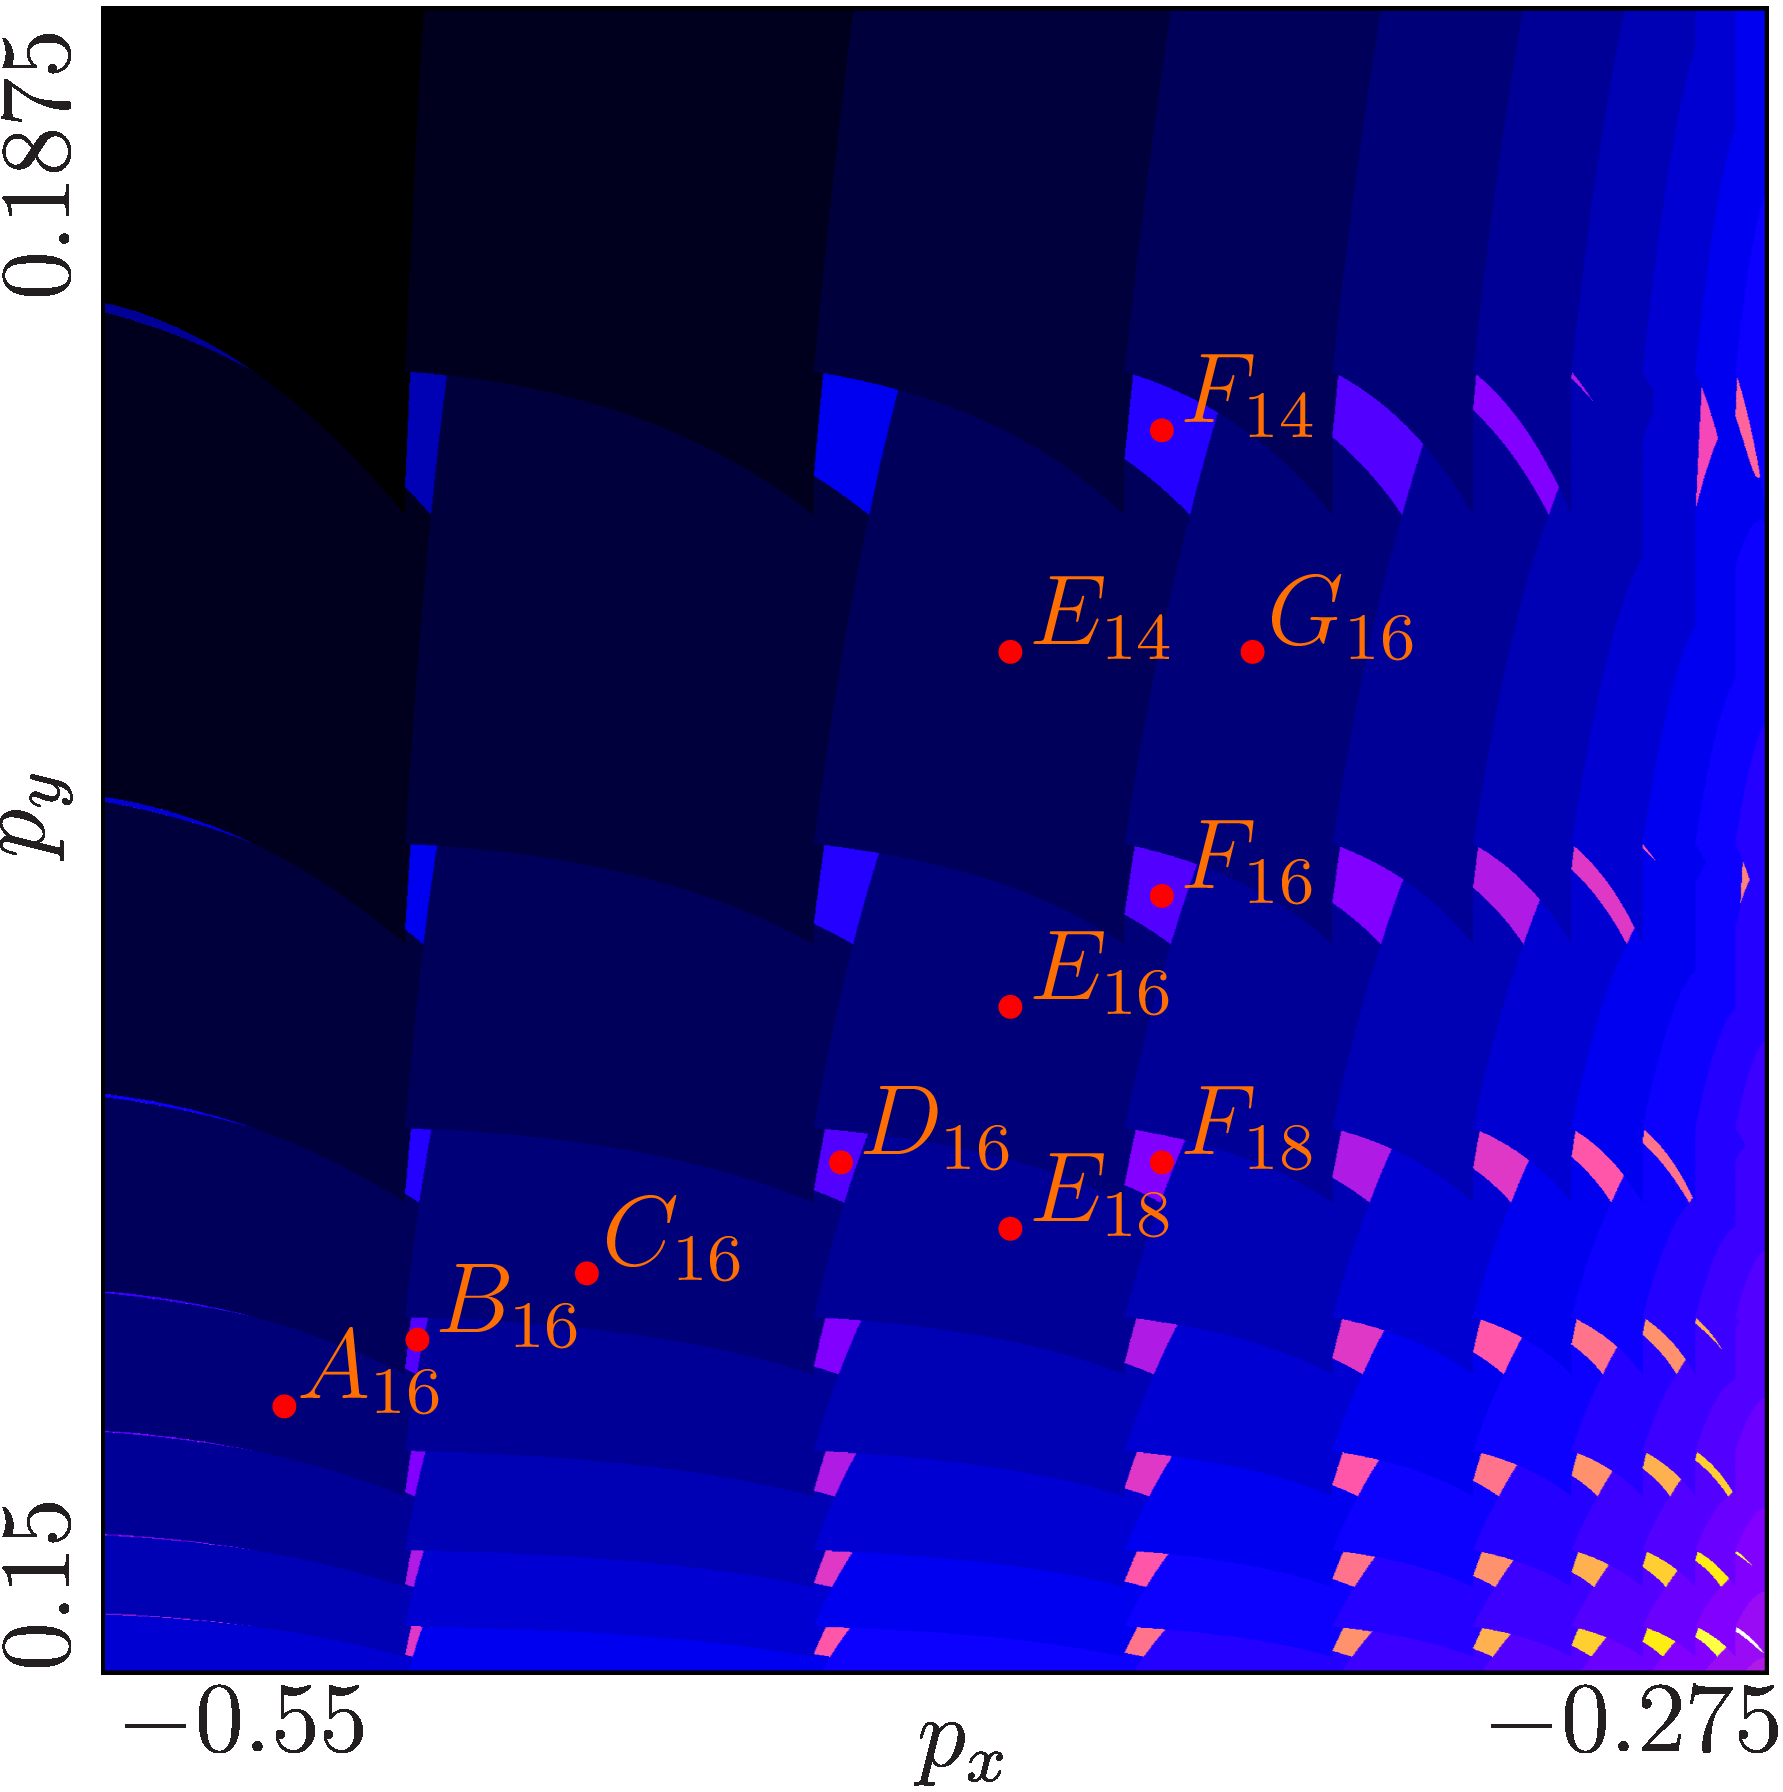
\includegraphics[width=\textwidth]{60_MinimalRepr/2D_Period_Whole_Lotta_Points/result-halved.png}
		\caption{Adjusted model}
		\label{fig:archdyn.dyn.period.halved}
	\end{subfigure}
	\caption[2D scan of the periods of the archetypal model]{
		2D scan of the periods of the archetypal model.
		The parameters $a_L = 4, b_L = -\frac{1}{2},$ and $g_R\left(\frac{1}{4}\right) = 0.525$ are fixed.
		The parameters $\alpha = -g_R\left(\frac{1}{4}\right)$ and $\beta = c_L$ are varied in the ranges $[-0.55, -0.275]$ and $[0.15, 0.1875]$, respectively.
		The points $A_{16}, B_{16}, C_{16}, D_{16}, E_{16},$ and $F_{16}$ mark the parameter values used for the cobweb diagrams in \Cref{fig:archdyn.dyn.cobwebs.1,fig:archdyn.dyn.cobwebs.2}.
		(a) shows the scan for the normal model as defined above, while (b) shows the scan for the adjusted model where we can see ``type B'' parameter regions.
	}
	\label{fig:archdyn.dyn.period}
\end{figure}

\todo{Period Figure: add periods, remove point $F_{14}$, $F_{16}$}

\begin{figure}
	\centering
	\begin{subfigure}{0.3\textwidth}
		\centering
		\includegraphics[width=\textwidth]{60_MinimalRepr/Cobweb_A16/result.png}
		\caption{At point $A_{16}$}
		\label{fig:archdyn.dyn.cobweb.A}
	\end{subfigure}
	\begin{subfigure}{0.3\textwidth}
		\centering
		\includegraphics[width=\textwidth]{60_MinimalRepr/Cobweb_B16/result.png}
		\caption{At point $B_{16}$}
		\label{fig:archdyn.dyn.cobweb.B}
	\end{subfigure}
	\begin{subfigure}{0.3\textwidth}
		\centering
		\includegraphics[width=\textwidth]{60_MinimalRepr/Cobweb_C16/result.png}
		\caption{At point $C_{16}$}
		\label{fig:archdyn.dyn.cobweb.C}
	\end{subfigure}
	\caption[Cobweb diagrams of the archetypal model]{
		Cobweb diagrams at three parameter values of $\alpha = -g_R\left(\frac{1}{4}\right)$ and $\beta = c_L$ in the archetypal model.
		The other parameters are fixed as $a_L = 4, b_L = -\frac{1}{2},$ and $g_R\left(\frac{1}{2}\right) = \frac{1}{2} + \frac{1}{40}$.
		The parameter values are marked as points $A_{16}, B_{16},$ and $C_{16}$ in \Cref{fig:archdyn.dyn.period}.
	}
	\label{fig:archdyn.dyn.cobwebs.1}
\end{figure}

As in \Citeauthor{akyuz2022}'s thesis, we will take a look at the chain of parameter regions which have stable cycles of period $16$.
The parameter regions are marked with the points $A_{16}$ to $F_{16}$ in \Cref{fig:archdyn.dyn.period}.
\Cref{fig:archdyn.dyn.cobwebs.1} shows cobwebs for the points $A_{16}, B_{16},$ and $C_{16}$.
The parameter region containing $A_{16}$ is denoted $\P_{\A^7\B\C^7\D}$ since its only stable cycle is $\Cycle{\A^7\B\C^7\D}$.
\Cref{fig:setup.og.dynamics.cobweb.A} shows the cobweb diagram of this cycle.
The parameter region, therefore, is a ``type A'' parameter region with only one stable cycle of period 16.
The next parameter region contains the point $B_{16}$ and has two stable cycles $\Cycle{\A^7\B\C^6\D^2}$ and $\Cycle{\A^6\B^2\C^7\D}$.
\Cref{fig:setup.og.dynamics.cobweb.B} shows the cobweb diagram of these two cycles.
The parameter region containing these cycles is denoted $\P_{\A^7\B\C^6\D^2, \A^6\B^2\C^7\D}$.
Per the same logic, the parameter region marked with point $C_{16}$ is denoted $\P_{\A^6\B^2\C^6\D^2}$.
\Cref{fig:archdyn.dyn.cobweb.C} shows the cobweb diagram of that cycle.

\begin{figure}
	\centering
	\begin{subfigure}{0.3\textwidth}
		\centering
		\includegraphics[width=\textwidth]{60_MinimalRepr/Cobweb_D16/result.png}
		\caption{At point $D_{16}$}
		\label{fig:archdyn.dyn.cobweb.D}
	\end{subfigure}
	\begin{subfigure}{0.3\textwidth}
		\centering
		\includegraphics[width=\textwidth]{60_MinimalRepr/Cobweb_E16/result.png}
		\caption{At point $E_{16}$}
		\label{fig:archdyn.dyn.cobweb.E}
	\end{subfigure}
	\begin{subfigure}{0.3\textwidth}
		\centering
		\includegraphics[width=\textwidth]{60_MinimalRepr/Cobweb_F16/result.png}
		\caption{At point $F_{16}$}
		\label{fig:archdyn.dyn.cobweb.F}
	\end{subfigure}
	\caption[Cobweb diagrams of the archetypal model]{
		Cobweb diagrams at three parameter values of $\alpha = -g_R\left(\frac{1}{4}\right)$ and $\beta = c_L$ in the archetypal model.
		The other parameters are fixed as $a_L = 4, b_L = -\frac{1}{2},$ and $g_R\left(\frac{1}{2}\right) = \frac{1}{2} + \frac{1}{40}$.
		The parameter values are marked as points $D_{16}, E_{16},$ and $F_{16}$ in \Cref{fig:archdyn.dyn.period}.
	}
	\label{fig:archdyn.dyn.cobwebs.2}
\end{figure}
\todo{Cobwebs of type B cycles: different color}

Thus far these parameter regions follow the rules laid out in \Citeauthor{akyuz2022}'s thesis and listed again in \Cref{sec:state.og.dynamics}~\Cite{akyuz2022}.
The first parameter region has the stable cycle $\Cycle{\A^{\frac{P}{2} - 1}\B\C^{\frac{P}{2} - 1}\D}$ where $P = 16$ is the period.
It is a ``type A'' parameter region and the next parameter region is of ``type B'', as the rules require.
This parameter region has the stable cycles $\Cycle{\A^{\frac{P}{2} - 1}\B\C^{\frac{P}{2} - 2}\D^2}$ and $\Cycle{\A^{\frac{P}{2} - 2}\B^2\C^{\frac{P}{2} - 1}\D}$.
This also agrees with the rules.
The next parameter region is of ``type A'' again and has the stable cycle $\Cycle{A^{\frac{P}{2} - 1}\B^2\C^{\frac{P}{2} - 2}\D^2}$ as expected by the rules.
This chain continues to abide by the rules as can be seen in the cobweb diagrams of points $D_{16}, E_{16},$ and $F_{16}$ in \Cref{fig:archdyn.dyn.cobwebs.2}.
The corresponding parameter regions are $\P_{\A^6\B^2\C^5\D^3, \A^5\B^3\C^6\D^2}, \P_{\A^5\B^3\C^5\D^3},$ and $\P_{\A^5\B^3\C^4\D^4, \A^4\B^4\C^5\D^3}$ respectively.

\begin{figure}
	\centering
	\begin{subfigure}{0.3\textwidth}
		\centering
		\includegraphics[width=\textwidth]{60_MinimalRepr/Cobweb_D16/result.png}
		\caption{At point $D_{16}$}
		\label{fig:archdyn.dyn.cobweb.D}
	\end{subfigure}
	\begin{subfigure}{0.3\textwidth}
		\centering
		\includegraphics[width=\textwidth]{60_MinimalRepr/Cobweb_E16/result.png}
		\caption{At point $E_{16}$}
		\label{fig:archdyn.dyn.cobweb.E}
	\end{subfigure}
	\begin{subfigure}{0.3\textwidth}
		\centering
		\includegraphics[width=\textwidth]{60_MinimalRepr/Cobweb_F16/result.png}
		\caption{At point $F_{16}$}
		\label{fig:archdyn.dyn.cobweb.F}
	\end{subfigure}
	\caption[Cobweb diagrams of the archetypal model]{
		Cobweb diagrams at three parameter values of $\alpha = -g_R\left(\frac{1}{4}\right)$ and $\beta = c_L$ in the archetypal model.
		The other parameters are fixed as $a_L = 4, b_L = -\frac{1}{2},$ and $g_R\left(\frac{1}{2}\right) = \frac{1}{2} + \frac{1}{40}$.
		The parameter values are marked as points $G_{16}, E_{14},$ and $E_{18}$ in \Cref{fig:archdyn.dyn.period}.
	}
	\label{fig:archdyn.dyn.cobwebs.3}
\end{figure}

The stable cycle in the parameter region marked with point $E_{14}$ has period $14$.
This agrees with the rule that the neighboring chains differ in their periods by 2.
Its symbolic sequence is $\A^4\B^3\C^4\D^3$ and its cobweb diagram can be seen in \Cref{fig:archdyn.dyn.cobweb.E14}.
Similarly, the symbolic sequence of the stable cycle in the parameter regions marked with $E_{16}$ has period $16$.
Its symbolic sequence is $\A^6\B^3\C^6\D^3$ and its cobweb diagram can be seen in \Cref{fig:archdyn.dyn.cobweb.E14}.
So the cycles in the ``type A'' regions directly above another ``type A'' parameter region with stable cycle $\Cycle{\A^a\B^b\C^a\D^b}$ has the stable cycle $\Cycle{\A^{a-1}\B^b\C^{a-1}\D^b}$.

We can also explore what rules apply to ``type A'' parameter regions that are horizontally next to each other.
The parameter region with point $C_{16}$ is directly left of the parameter region with point $E_{18}$.
It has the stable cycle $\Cycle{\A^6\B^2\C^6\D^2}$, while the parameter region with point $E_{18}$ has the stable cycle $\Cycle{\A16\B^3\C^6\D^3}$.
Similarly, the stable cycle in the parameter region marked with point $G_{16}$ which is directly right of paramater region marked with point $E_{14}$ that has the stable cycle $\Cycle{\A^4\B^4\C^4\D^4}$, has the stable cycle $\Cycle{\A^4\B^3\C^4\D^3}$
Therefore, the cycles in the ``type A'' regions directly left of another ``type A'' parameter region with stable cycle $\Cycle{\A^a\B^b\C^a\D^b}$ has the stable cycle $\Cycle{\A^a\B^{b-1}\C^a\D^{b-1}}$.
The cobweb diagrams for the cycles at points $E_{14}, E_{18},$ and $G_{16}$ are shown in \Cref{fig:archdyn.dyn.cobwebs.3}.

\todo{Cobweb diagrams for $E_{14}$, $E_{18}$, and $G_{16}$}
